\documentclass{report}
%\usepackage[utopia]{mathdesign}
%\usepackage{amsmath, amsthm}
\usepackage{pgfplots}


\usepackage{amsmath,amsfonts,amsthm,amssymb,mathtools}
%\usepackage[varbb]{newpxmath}
%\usepackage[osf,largesc,theoremfont]{newpxtext}
%\usepackage{coelacanth}
%\usepackage{beraserif} % Bitstream Vera Serif font
%\usepackage{berasans} % Bitstream Vera Sans font
%\usepackage{beramono} % Bitstream Vera Sans Mono font
%\usepackage{berasans}
%\usepackage{libertine}
%\usepackage{mathpazo}
%\usepackage{palatino}
%\usepackage{crimson}


%% Choose one of the following (if not choosing the  
%% default, viz., Computer Modern, font family):
%\usepackage{lmodern}
\usepackage{bold-extra}
%%
%\usepackage{mathpazo}
% \usepackage{newpxmath}
%\usepackage{kpfonts} % Very good
%%
%\usepackage{mathptmx} %Very good
%\usepackage{stix} 
%\usepackage{txfonts} %Very good
\usepackage{newtxtext,newtxmath} %Very good
%%
%\usepackage{libertine} \usepackage[libertine]{newtxmath}
%\usepackage{libertine,libertinust1math} % added 2019/11/28
%%
%\usepackage{newpxtext} 
%\usepackage{breqn} 
\usepackage[euler-digits]{eulervm}
%\usepackage{textcomp}
%\usepackage{bm}
\usepackage{contour}
\usepackage{adjustbox}






\input{/home/cryptopsy/Semesters/LaTeXTemplates/UniversalTeXTemplate/preamble.tex}
%From M275 "Topology" at SJSU
\newcommand{\id}{\mathrm{id}} % Identité
\newcommand{\taking}[1]{\xrightarrow{#1}} % Flèche avec annotation
\newcommand{\inv}{^{-1}} % Inverse

%From M170 "Introduction to Graph Theory" at SJSU
\DeclareMathOperator{\diam}{diam} % Diamètre
\DeclareMathOperator{\ord}{ord} % Ordre
\newcommand{\defeq}{\overset{\mathrm{def}}{=}} % Défini comme égal

%From the USAMO .tex files
\newcommand{\ts}{\textsuperscript} % Exposant
\newcommand{\dg}{^\circ} % Degré
\newcommand{\ii}{\item} % Item

% % From Math 55 and Math 145 at Harvard
% \newenvironment{subproof}[1][Proof]{%
% \begin{proof}[#1] \renewcommand{\qedsymbol}{$\blacksquare$}}%
% {\end{proof}}

\newcommand{\liff}{\leftrightarrow} % Si et seulement si
\newcommand{\lthen}{\rightarrow} % Implique
\newcommand{\opname}{\operatorname} % Opérateur générique
\newcommand{\surjto}{\twoheadrightarrow} % Flèche surjective
\newcommand{\injto}{\hookrightarrow} % Flèche injective
\newcommand{\On}{\mathrm{On}} % Ordinaux
\DeclareMathOperator{\img}{im} % Image
\DeclareMathOperator{\Img}{Im} % Image
\DeclareMathOperator{\coker}{coker} % Cokernel
\DeclareMathOperator{\Coker}{Coker} % Cokernel
\DeclareMathOperator{\Ker}{Ker} % Noyau
\DeclareMathOperator{\rank}{rank} % Rang
\DeclareMathOperator{\Spec}{Spec} % Spectre
\DeclareMathOperator{\Tr}{Tr} % Trace
\DeclareMathOperator{\pr}{pr} % Projection
\DeclareMathOperator{\ext}{ext} % Extension
\DeclareMathOperator{\pred}{pred} % Prédécesseur
\DeclareMathOperator{\dom}{dom} % Domaine
\DeclareMathOperator{\ran}{ran} % Image (range)
\DeclareMathOperator{\Hom}{Hom} % Homomorphisme
\DeclareMathOperator{\Mor}{Mor} % Morphismes
\DeclareMathOperator{\End}{End} % Endomorphisme

\newcommand{\eps}{\epsilon} % Épsilon
\newcommand{\veps}{\varepsilon} % Variance d'épsilon
\newcommand{\ol}{\overline} % Ligne au-dessus
\newcommand{\ul}{\underline} % Ligne en-dessous
\newcommand{\wt}{\widetilde} % Tilde large
\newcommand{\wh}{\widehat} % Chapeau large
\newcommand{\vocab}[1]{\textbf{\color{blue} #1}} % Texte en gras et bleu
\providecommand{\half}{\frac{1}{2}} % Fraction 1/2
\newcommand{\dang}{\measuredangle} % Angle dirigé
\newcommand{\ray}[1]{\overrightarrow{#1}} % Ray
\newcommand{\seg}[1]{\overline{#1}} % Segment
\newcommand{\arc}[1]{\wideparen{#1}} % Arc
\DeclareMathOperator{\cis}{cis} % cis
\DeclareMathOperator*{\lcm}{lcm} % Plus petit commun multiple
\DeclareMathOperator*{\argmin}{arg min} % Argument du minimum
\DeclareMathOperator*{\argmax}{arg max} % Argument du maximum
\newcommand{\cycsum}{\sum_{\mathrm{cyc}}} % Somme cyclique
\newcommand{\symsum}{\sum_{\mathrm{sym}}} % Somme symétrique
\newcommand{\cycprod}{\prod_{\mathrm{cyc}}} % Produit cyclique
\newcommand{\symprod}{\prod_{\mathrm{sym}}} % Produit symétrique
\newcommand{\Qed}{\begin{flushright}\qed\end{flushright}} % QED aligné à droite
\newcommand{\parinn}{\setlength{\parindent}{1cm}} % Indentation de paragraphe à 1 cm
\newcommand{\parinf}{\setlength{\parindent}{0cm}} % Pas d'indentation de paragraphe
% \newcommand{\norm}{\|\cdot\|} % Norme
\newcommand{\inorm}{\norm_{\infty}} % Norme infinie
\newcommand{\opensets}{\{V_{\alpha}\}_{\alpha\in I}} % Ensemble ouvert
\newcommand{\oset}{V_{\alpha}} % Ensemble ouvert V
\newcommand{\opset}[1]{V_{\alpha_{#1}}} % Ensemble ouvert V avec indice
\newcommand{\lub}{\text{lub}} % Plus petite borne supérieure
\newcommand{\del}[2]{\frac{\partial #1}{\partial #2}} % Dérivée partielle
\newcommand{\Del}[3]{\frac{\partial^{#1} #2}{\partial^{#1} #3}} % Dérivée partielle d'ordre élevé
\newcommand{\deld}[2]{\dfrac{\partial #1}{\partial #2}} % Dérivée partielle avec dfrac
\newcommand{\Deld}[3]{\dfrac{\partial^{#1} #2}{\partial^{#1} #3}} % Dérivée partielle d'ordre élevé avec dfrac
\newcommand{\lm}{\lambda} % Lambda
\newcommand{\uin}{\mathbin{\rotatebox[origin=c]{90}{$\in$}}} % Appartient, tourné de 90 degrés
\newcommand{\usubset}{\mathbin{\rotatebox[origin=c]{90}{$\subset$}}} % Sous-ensemble, tourné de 90 degrés
\newcommand{\lt}{\left} % Gauche
\newcommand{\rt}{\right} % Droite
\newcommand{\bs}[1]{\boldsymbol{#1}} % Symbole en gras
\newcommand{\exs}{\exists} % Il existe
\newcommand{\st}{\strut} % Strut
\newcommand{\dps}[1]{\displaystyle{#1}} % Disposition en ligne

\newcommand{\sol}{\setlength{\parindent}{0cm}\textbf{\textit{Solution:}}\setlength{\parindent}{1cm} } % Solution sans indentation initiale puis rétablie
\newcommand{\solve}[1]{\setlength{\parindent}{0cm}\textbf{\textit{Solution: }}\setlength{\parindent}{1cm}#1 \Qed}

\newcommand{\entoure}[1]{\fcolorbox{black}{gray!30}{\texttt{#1}}}

\renewcommand{\ttdefault}{cmtt}
\newcommand{\textttbf}[1]{\contour{yellow!45}{\texttt{#1}}}
\newcommand{\varitem}[3][black]{%
    \item [%
        \colorbox{#2}{\textcolor{#1}{\makebox(5.5,7){#3}}}%
    ]
}
% Allow you to do the non implication (implication barred)
\newcommand{\notimplies}{%
  \mathrel{{\ooalign{\hidewidth$\not\phantom{=}$\hidewidth\cr$\implies$}}}}


\newcommand*{\authorimg}[1]%
    { \raisebox{-1\baselineskip}{\includegraphics[width=\imagesize]{#1}}}
\newlength\imagesize 

\input{/home/cryptopsy/Semesters/LaTeXTemplates/UniversalTeXTemplate/letterfonts.tex}
% lstlistingsEnvs.tex

\usepackage{minted}


\lstset{
  basicstyle=\ttfamily, % Set
  columns=fullflexible,
  keepspaces=true,
  language=Python % You can specify the language if you want syntax highlighting
}

%%%%%%%%%%%%%%%%%%%%%%%%%%%%%%%%%%%%%%%%%%%%%%%%%%%%%%%%%%%%%%%%%%%%%%%%%%%%%%%%%%%%%%%%%%%%%%%%%
%                                 Custom lstlisting Environments
%%%%%%%%%%%%%%%%%%%%%%%%%%%%%%%%%%%%%%%%%%%%%%%%%%%%%%%%%%%%%%%%%%%%%%%%%%%%%%%%%%%%%%%%%%%%%%%%%
% Gruvbox style for Python
\definecolor{Pgruvbox-bg}{HTML}{282828}
\definecolor{Pgruvbox-fg}{HTML}{ebdbb2}
\definecolor{Pgruvbox-red}{HTML}{fb4934}
\definecolor{Pgruvbox-green}{HTML}{b8bb26}
\definecolor{Pgruvbox-yellow}{HTML}{fabd2f}
\definecolor{Pgruvbox-blue}{HTML}{83a598}
\definecolor{Pgruvbox-purple}{HTML}{d3869b}
\definecolor{Pgruvbox-aqua}{HTML}{8ec07c}
\definecolor{BBBlack}{rgb}{0.05, 0.06, 0.09}



% JAVA LSTLISTING STYLE IN Gruvbox Colorscheme
\definecolor{gruvbox-bg}{rgb}{0.282, 0.247, 0.204}
\definecolor{gruvbox-fg1}{rgb}{0.949, 0.898, 0.776}
\definecolor{gruvbox-fg2}{rgb}{0.871, 0.804, 0.671}
\definecolor{gruvbox-red}{rgb}{0.788, 0.255, 0.259}
\definecolor{gruvbox-green}{rgb}{0.518, 0.604, 0.239}
\definecolor{gruvbox-yellow}{rgb}{0.914, 0.808, 0.427}
\definecolor{gruvbox-blue}{rgb}{0.353, 0.510, 0.784}
\definecolor{gruvbox-purple}{rgb}{0.576, 0.412, 0.659}
\definecolor{gruvbox-aqua}{rgb}{0.459, 0.631, 0.737}
\definecolor{gruvbox-gray}{rgb}{0.518, 0.494, 0.471}

\definecolor{lst-bg}{RGB}{45, 45, 45}
\definecolor{lst-fg}{RGB}{220, 220, 204}
\definecolor{lst-keyword}{RGB}{215, 186, 125}
\definecolor{lst-comment}{RGB}{117, 113, 94}
\definecolor{lst-string}{RGB}{163, 190, 140}
\definecolor{lst-number}{RGB}{181, 206, 168}
\definecolor{lst-type}{RGB}{218, 142, 130}

\lstdefinestyle{PythonGruvbox}{
    language=Python,
    identifierstyle=\color{lst-fg},
    basicstyle=\ttfamily\color{Pgruvbox-fg},
    keywordstyle=\color{Pgruvbox-yellow},
    keywordstyle=[2]\color{Pgruvbox-blue},
    stringstyle=\color{Pgruvbox-green},
    commentstyle=\color{Pgruvbox-aqua},
    backgroundcolor=\color{BBBlack},
    rulecolor=\color{BBBlack},
    showstringspaces=false,
    keepspaces=true,
    captionpos=b,
    breaklines=true,
    tabsize=4,
    showspaces=false,
    numbers=left,
    numbersep=5pt,
    numberstyle=\tiny\color{gray},
    showtabs=false,
    columns=fullflexible,
    morekeywords={True,False,None},
    morekeywords=[2]{and,as,assert,break,class,continue,def,del,elif,else,except,exec,
    finally,for,from,global,if,import,in,is,lambda,nonlocal,not,or,pass,print,raise,
    return,try,while,with,yield},
    morecomment=[s]{"""}{"""},
    morecomment=[s]{'''}{'''},
    morecomment=[l]{\#},
    morestring=[b]",
    morestring=[b]',
    literate=
    {0}{{\textcolor{Pgruvbox-purple}{0}}}{1}
    {1}{{\textcolor{Pgruvbox-purple}{1}}}{1}
    {2}{{\textcolor{Pgruvbox-purple}{2}}}{1}
    {3}{{\textcolor{Pgruvbox-purple}{3}}}{1}
    {4}{{\textcolor{Pgruvbox-purple}{4}}}{1}
    {5}{{\textcolor{Pgruvbox-purple}{5}}}{1}
    {6}{{\textcolor{Pgruvbox-purple}{6}}}{1}
    {7}{{\textcolor{Pgruvbox-purple}{7}}}{1}
    {8}{{\textcolor{Pgruvbox-purple}{8}}}{1}
    {9}{{\textcolor{Pgruvbox-purple}{9}}}{1}
}

% Gruvbox style for Java
\definecolor{gruvbox-bg}{rgb}{0.282, 0.247, 0.204}
\definecolor{gruvbox-fg1}{rgb}{0.949, 0.898, 0.776}
\definecolor{gruvbox-fg2}{rgb}{0.871, 0.804, 0.671}
\definecolor{gruvbox-red}{rgb}{0.788, 0.255, 0.259}
\definecolor{gruvbox-green}{rgb}{0.518, 0.604, 0.239}
\definecolor{gruvbox-yellow}{rgb}{0.914, 0.808, 0.427}
\definecolor{gruvbox-blue}{rgb}{0.353, 0.510, 0.784}
\definecolor{gruvbox-purple}{rgb}{0.576, 0.412, 0.659}
\definecolor{gruvbox-aqua}{rgb}{0.459, 0.631, 0.737}
\definecolor{gruvbox-gray}{rgb}{0.518, 0.494, 0.471}

\lstdefinestyle{JavaGruvbox}{
    language=Java,
    basicstyle=\ttfamily\color{Pgruvbox-fg},
    keywordstyle=\color{Pgruvbox-yellow},
    keywordstyle=[2]\color{lst-type},
    commentstyle=\itshape\color{lst-comment},
    stringstyle=\color{lst-string},
    numberstyle=\color{lst-number},
    backgroundcolor=\color{BBBlack},
    rulecolor=\color{gruvbox-aqua},
    showstringspaces=false,
    keepspaces=true,
    captionpos=b,
    breaklines=true,
    tabsize=4,
    showspaces=false,
    showtabs=false,
    columns=fullflexible,
    morekeywords={var},
    morekeywords=[2]{boolean, byte, char, double, float, int, long, short, void},
    morecomment=[s]{/}{/},
    morecomment=[l]{//},
    morestring=[b]",
    morestring=[b]',
    numbers=left,
    numbersep=5pt,
    numberstyle=\tiny\color{gray},
}

% Dracula style for Java
\definecolor{draculawhite-background}{RGB}{237, 239, 252}
\definecolor{draculawhite-comment}{RGB}{98, 114, 164}
\definecolor{draculawhite-keyword}{RGB}{189, 147, 249}
\definecolor{draculawhite-string}{RGB}{152, 195, 121}
\definecolor{draculawhite-number}{RGB}{249, 189, 89}
\definecolor{draculawhite-operator}{RGB}{248, 248, 242}

\lstdefinestyle{JavaDraculaWhite}{
    language=Java,
    backgroundcolor=\color{draculawhite-background},
    commentstyle=\itshape\color{draculawhite-comment},
    keywordstyle=\color{draculawhite-keyword},
    stringstyle=\color{draculawhite-string},
    basicstyle=\ttfamily\footnotesize\color{black},
    identifierstyle=\color{black},
    keywordstyle=\color{draculawhite-keyword}\bfseries,
    morecomment=[s][\color{draculawhite-comment}]{/**}{*/},
    showstringspaces=false,
    showspaces=false,
    breaklines=true,
    %frame=single,
    rulecolor=\color{draculawhite-operator},
    tabsize=2,  
    numbers=left,
    numbersep=4pt,
    numberstyle=\ttfamily\tiny\color{gray}
}

% Dracula style for Python
\definecolor{draculawhite-bg}{HTML}{FAFAFA}
\definecolor{draculawhite-fg}{HTML}{282A36}
\definecolor{pdraculawhite-keyword}{HTML}{BD93F9}
\definecolor{pdraculawhite-comment}{HTML}{6272A4}
\definecolor{draculawhite-number}{HTML}{FF79C6}

\lstdefinestyle{PythonDraculaWhite}{
    language=Python,
    basicstyle=\ttfamily\small\color{draculawhite-fg},
    backgroundcolor=\color{draculawhite-background},
    keywordstyle=\color{orange}\bfseries,
    stringstyle=\color{draculawhite-string},
    commentstyle=\color{pdraculawhite-comment}\itshape,
    numberstyle=\color{draculawhite-number},
    showstringspaces=false,
    showspaces=false,
    breaklines=true,
    frame=single,
    rulecolor=\color{draculawhite-operator}, 
    tabsize=4,
    morekeywords={as,with,1,2,3,4, 5,6,7,8,9,True,False},
    numbers=left,
    numbersep=5pt,
    numberstyle=\small\bfseries\ttfamily\color{htmlcomment},
}

% Dracula Dark style for HTML
\definecolor{htmltag}{HTML}{ff79c6}
\definecolor{htmlattr}{HTML}{f1fa8c}
\definecolor{htmlvalue}{HTML}{bd93f9}
\definecolor{htmlcomment}{HTML}{6272a4}
\definecolor{htmltext}{HTML}{401E31}
\definecolor{htmlbackground}{HTML}{282a36}
\definecolor{comphtmlbackground}{HTML}{8093FF}

\lstdefinestyle{HTMLDraculaDark}{
    basicstyle=\normalsize\bfseries\ttfamily\color{htmltext},
    commentstyle=\itshape\color{htmlcomment},
    keywordstyle=\bfseries\color{htmltag},
    stringstyle=\color{htmlvalue},
    emph={DOCTYPE,html,head,body,div,span,a,script},
    emphstyle={\color{htmltag}\bfseries},
    sensitive=true,
    showstringspaces=false,
    backgroundcolor=\color{white},
    inputencoding=utf8,
    extendedchars=true,
    language=HTML,
    tabsize=4,
    breaklines=true,
    breakatwhitespace=true,
    numbers=left,
    numbersep=10pt,
    numberstyle=\small\bfseries\ttfamily\color{htmlcomment},
    escapeinside={<@}{@>},
    rulecolor=\color{htmlbackground},
    xleftmargin=10pt,
    frame=none, 
    breaklines=true,
    postbreak=\mbox{\textcolor{gray}{$\hookrightarrow$}\space},
    showlines=false,
    moredelim=[s][\itshape\color{htmlcomment}]{<!--}{-->},
    morekeywords={id,class,type,name,value,placeholder,checked,src,href,alt},
    literate={é}{{\'e}}1 {è}{{\`e}}1 {ê}{{\^e}}1 {ë}{{\"e}}1 {à}{{\`a}}1 {ù}{{\`u}}1 {û}{{\^u}}1 {ç}{{\c{c}}}1 {â}{{\^a}}1 {î}{{\^i}}1 {ï}{{\"i}}1
}


\lstdefinestyle{Haskell}{
  frame=none,
  xleftmargin=2pt,
  stepnumber=1,
  numbers=left,
  numbersep=5pt,
  numberstyle=\ttfamily\tiny\color[gray]{0.3},
  belowcaptionskip=\bigskipamount,
  captionpos=b,
  escapeinside={*'}{'*},
  language=haskell,
  tabsize=2,
  emphstyle={\bf},
  %commentstyle=\it,
  stringstyle=\mdseries\ttfamily,
  showspaces=false,
  keywordstyle=\bfseries\ttfamily,
  columns=flexible,
  basicstyle=\small\ttfamily,
  showstringspaces=false,
  morecomment=[l]\%,
}



\lstdefinestyle{CSSDraculaLight}{
    basicstyle=\bfseries\scriptsize\ttfamily\color{htmltext},
    commentstyle=\color{htmlcomment},
    keywordstyle=\bfseries\color{htmlvalue},
    stringstyle=\color{htmlvalue},
    emph={DOCTYPE,html,head,body,div,span,a,script},
    emphstyle={\color{htmltag}\bfseries},
    sensitive=true,
    showstringspaces=false,
    backgroundcolor=\color{white},
    inputencoding=utf8,
    extendedchars=true, % Support extended characters
    frame=none, 
    %frame=tb,
    tabsize=4,
    breaklines=true,
    breakatwhitespace=true,
    numbers=left,
    numbersep=10pt,
    numberstyle=\small\bfseries\ttfamily\color{htmlcomment},
    escapeinside={<@}{@>},
    rulecolor=\color{htmlbackground},
    xleftmargin=20pt,
    % Add a vertical line for opening and closing tags
    %frame=lines,
    framesep=2pt,
    framexleftmargin=4pt,
    % Add a vertical line for closing tags that go through multiple lines
    breaklines=true,
    postbreak=\mbox{\textcolor{gray}{$\hookrightarrow$}\space},
    showlines=true,
    % Add a rule to apply commentstyle to keywords inside comments
    moredelim=[s][\color{htmlcomment}]{/*}{*/},
    literate={é}{{\'e}}1
             {è}{{\`e}}1
             {ê}{{\^e}}1
             {ë}{{\"e}}1
             {à}{{\`a}}1
             {ù}{{\`u}}1
             {û}{{\^u}}1
             {ç}{{\c{c}}}1
             {â}{{\^a}}1
             {î}{{\^i}}1
             {ï}{{\"i}}1,
    morekeywords={color, background, background-color, font-size, font-weight, border, border-radius, padding, margin, display, position, top, right, bottom, left, flex, grid, width, height, min-width, max-width, min-height, max-height, transition, transform, animation, keyframes, content, z-index,id,class,type,name,value,placeholder,checked,src,href,alt},
    morestring=[s][\color{htmltag}]{:}{;},
}












\title{\huge{MATH1400}\\\Huge{Calcul à plusieurs variables}\\\vspace{2em}Travail Pratique 1 }
\author{\huge{Franz Girardin}}
\date{\today}


   

\begin{document}

\maketitle
\newpage% or \cleardoublepage
% \pdfbookmark[<level>]{<title>}{<dest>}
\pdfbookmark[section]{\contentsname}{toc}
\tableofcontents
\pagebreak


\titleformat*{\section}{%
    \normalsize\bfseries%
}

\titleformat{\section}[block]{\normalsize\bfseries}{}{0pt}{}


    \chapter*{Exercices sur les suite numériques}
  \section{Définition de convergence}
  \begin{Exercice}{(Stewart 1.1.2)}{}
      Qu'est-ce qu'une \textit{suite convergente} ? Donnez \textbf{deux exemples}. 
      Qu'est-ce qu'une \textit{suite divergente} ? Donnez \textbf{deux} exemples   
  \end{Exercice}

  Est \textcolor{myb}{\textbf{convergente}} 
  toute \textbf{suite} $\{a_n\}$ dont les termes $a_n$ 
  s'approchent autant 
  que l'on veut d'une valeur $L$ lorsque l'entier $n$ devient arbitrairement grand : 

  \begin{align*}
      \left(\lim\limits_{n\to\infty}a_n = L\right) \implies a_n \; \textcolor{myb}{\textbf{conv}}.    
  \end{align*}

  Plus formellement, soit une valeur positive arbitrairement petite $\varepsilon$, 
  il existe toujours un entier $N(\varepsilon)$ qui représente un rang 
  à partir duquel s'il y a un entier naturel $n > N(\varepsilon)$, \textbf{alors}
  l'image de cet entier naturel, $a_n$ sera aussi proche que l'on veut d'une 
  \textbf{valeur} $L$ représentant \textit{le point de convergence de la suite} :

  \begin{align*}
    \forall \varepsilon > 0 : \exists N(\varepsilon) > 0 : 
    n > N \implies |a_n - L| < \varepsilon
  \end{align*}

    \textbf{Exemple de suites convergentes} : 
    $\{a_n \} = \dfrac{1}{n}, \quad% 
    \{b_n\} = \dfrac{1}{n^2}$   


    \vspace{2em}
    Est \textcolor{myr}{\textbf{divergente}} toute suite dont les termes $a_n$ ne 
    convergent vers acune valeur particulière; ils s'approchent plutôt 
    de $\pm \infty$ :

      \begin{align*}
          \left(\lim\limits_{n\to\infty}a_n = \pm \infty \right) \implies 
          a_n \; \textcolor{myr}{\textbf{div}}.    
      \end{align*}

    Plus formellement, soit un nombre positif arbitrairement grand $M > 0$, 
    on pourra toujours trouver une valeur $N(M) \in \mathbb{N}$ à partir duquel tous les 
    entiers $n > M$ auront une image $a_n$ \textbf{plus grande} 
    que nombre arbitrairement 
    grand. Cela signifie que les termes de la suites ne s'approchent d'aucune 
    valeur. 

    \begin{align*}
    \forall \; M > 0 : \exists N(M) \in \mathbb{N} > 0 : n > N 
    \implies a_n > M (\textcolor{myr}{\textbf{div}}. \; \textbf{+}\infty ) 
    \end{align*}

    
    \section{Identification des termes}
    \begin{Exercice}{(Stewart 1.1.8)}{}
        Donnez les \textbf{cinq premiers termes} de la suite 
        $a_{n}=\frac{\left(-1\right)^{n}n}{n!+1}$ 
    \end{Exercice}


    \begin{align*}
        a_1 = -\dfrac{1}{2}, \; a_2 = \dfrac{2}{3}, \; 
        a_3 = -\dfrac{3}{7}, \; 
        a_4 = \dfrac{4}{25} 
        a_5 = -\dfrac{5}{121} 
    \end{align*}                


    \begin{Exercice}{(Stewart 1.1.11)}{}
        Donnez les \textbf{cinq premiers termes} de la suite 
        $a_n = 2, \; a_{n+1} = \dfrac{a_n}{1 + a_n}$
    \end{Exercice}              


    \begin{align*}
        a_1 = \textcolor{myb}{2}, \; a_2 = \textcolor{myb}{\dfrac{2}{3}}, \; 
        a_3 = \dfrac{2}{3} \times \dfrac{3}{5} = \textcolor{myb}{\dfrac{2}{5}}, \; 
        a_4 = \dfrac{2}{5} \times \dfrac{5}{7}  = \textcolor{myb}{\dfrac{2}{7}}, \;
        a_5 = \dfrac{2}{7} \times \dfrac{7}{9} = \textcolor{myb}{\dfrac{2}{9}}
    \end{align*}    


    \section{Trouver la règle}
    \begin{Exercice}{(Stewart 1.1.15)}{}
       Trouver la formule du \textbf{terme général} $a_n$ de la suite    
       $\left\{-3, 2,-\frac43, \frac89, -\frac{16}{27},\ldots\right\}$ 
    \end{Exercice}              


    \begin{align*}
        a_n = \dfrac{(-1)^n 2^{n-1}}{3^{n - 2}}
    \end{align*}            


    \begin{Exercice}{(Stewart 1.1.18)}{}
    Trouver la formule du \textbf{terme général} $a_n$ de la suite    
    $\left\{1,0,-1,0,1,0,-1,0,\cdots \right\}$
    \end{Exercice}

    \begin{align*}
        a_n = \sin\left(\dfrac{n\pi}{2}\right)
    \end{align*}        

    \section{Estimer un somme}


    \begin{Exercice}{(Stewart 1.1.19 - 1.1.22)}{}
        Calculez, \textbf{à la quatrième décimale}, 
        les dix premiers termes de la suite et 
        utilisez-les pour tracer le graphique de la suite à la main. 
        La suite semble-t-elle avoir une limite ? 
        Si oui, \textbf{calculez cette limite}. 
        Si non, expliquez pourquoi.
    \end{Exercice}

    \vspace{1em}%
    \noindent\textbf{1.1.19}  $a_n = \dfrac{3n}{1 + 6n}$ 


    \begin{align*}
        a_1 = 0.4286, \; a_2 = 0.4615, \; 
        a_3 = 0.4736, \; a_4 = 0.4800, \; 
        a_5 = 0.4838, \;
        \\
        a_6 = 0.4864, \; a_7 = 0.4883, \; 
        a_8 = 0.4998, \; a_9 =0.4909, \; 
        a_{10} = 0.4918
    \end{align*}    


    \begin{center}
    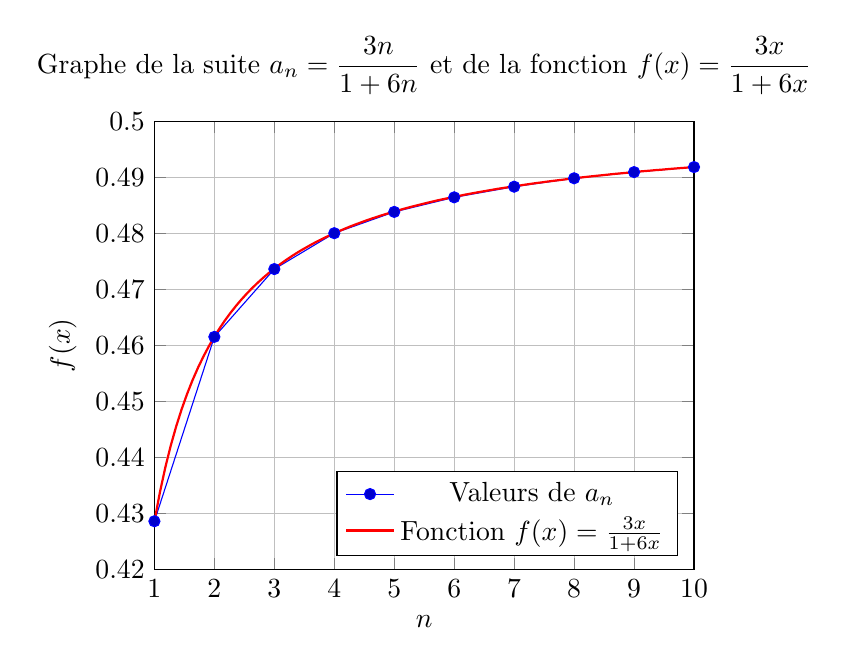
\begin{tikzpicture}
        \begin{axis}[
            title={Graphe de la suite $a_n = \dfrac{3n}{1 + 6n}$ 
            et de la fonction $f(x) =\dfrac{3x}{1 + 6x}$ },
            xlabel={$n$},
            ylabel={$f(x)$},
            grid=major,
            xmin=1, xmax=10,
            ymin=0.42, ymax=0.5,
            xtick={1,2,...,10},
            ytick={0.42, 0.43, 0.44, 0.45, 0.46, 0.47, 0.48, 0.49, 0.50},
            legend pos=south east
        ]
        
        % Plot des valeurs des dix premiers termes donnés
        \addplot coordinates {
            (1, 0.4286)
            (2, 0.4615)
            (3, 0.4736)
            (4, 0.4800)
            (5, 0.4838)
            (6, 0.4864)
            (7, 0.4883)
            (8, 0.4898)
            (9, 0.4909)
            (10, 0.4918)
        };
        \addlegendentry{Valeurs de $a_n$}

        % Tracé de la fonction a_n = 3n / (1 + 6n)
        \addplot[domain=1:10, samples=100, thick, red] 
        {3*x / (1 + 6*x)};
        \addlegendentry{Fonction $f(x) = \frac{3x}{1 + 6x}$}

        \end{axis}
    \end{tikzpicture}

    \end{center}


    \section{Déterminer la convergence}

    \begin{Exercice}{(Stewart 1.1.23 - 1.1.56)}{}
    Déterminez si la suite converge ou diverge. Si elle 
    converge, \textbf{trouvez sa limite}.       
    \end{Exercice}      




    \noindent\textbf{1.1.23}  $a_n = \dfrac{3 + 5n^2}{n + n^2}$  
    \vspace{1em}
    \noindent 
    $\lim\limits_{n\to+\infty }a_n \implies \textcolor{red}{\dfrac{\infty }{\infty }}$. 

    \begin{align*}
        \dfrac{3 + 5n^2}{n + n^2} = 
        \dfrac{n^2(\frac{1}{3n²} + 5)}{n^2(1+ \frac{1}{n})} = a_n \quad \text{(Simplifié)}
    \end{align*}

    \begin{align*}
        \lim\limits_{n \to+\infty }a_n  = 
        \lim\limits_{n \to+\infty }\dfrac{5  + \frac{1}{n}
        \cancelto{0}{\frac{1}{n}}}{1 + \cancelto{0}{\frac{1}{n}}}  =
        \lim\limits_{n \to+\infty } \frac{5}{1} = \dfrac{5}{1} 
    \end{align*}



    \noindent\textbf{1.1.42}  $a_n = \dfrac{\cos^{2}n}{n}$  
    \vspace{1em}

    Nous savons que la fonction $a_n$ est bornée entre les valeurs
    $\cos^{2}n \in [0, 1]$. Ainsi, pour tout $n \in \mathbb{N}$ 
    nous avons les équivalences suivantes : 

    \begin{align*}G
        0 \leq cos^{2}n  \leq 1 \\ 
        \dfrac{0}{n} \leq \dfrac{cos^{2} n}{n}  \leq \dfrac{1}{n}\\ 
        \lim\limits_{n \to+\infty }\cancelto{0}{\dfrac{0}{n}} \leq  
        \lim\limits_{n \to+\infty }\dfrac{cos^{2} n}{n} \leq 
        \lim\limits_{n \to+\infty }\cancelto{0}{\dfrac{1}{n}}
    \end{align*}

    Ainsi nous savons que la limite est bornée 
    \textbf{inférieurement et supérieurement} 
    par zéro, lorsque $n \longrightarrow \infty$. Ainsi, nous pouvons conclure 
    que la limite est égale à zéro et que la suite $a_n$ converge vers 
    $L = 0$. 

        
    \vspace{1em}%
    \noindent\textbf{1.1.44}  $a_n = \sqrt[n]{2^{1 + 3n}}$

    \begin{align*}
        a_n 
        = \sqrt[n]{2^{1 + 3n}} 
        = \left(2 \cdot 2^{3n} \right)^{\frac{1}{n}}
        = 2^{\frac{1}{n}} \cdot 2^{\frac{3n}{n}} \quad \text{(Développé)} \\ 
        \lim\limits_{n \to+\infty }a_n 
        = 
        \lim\limits_{n \to+\infty }  
        = 
        2^{\cancelto{0}{\frac{1}{n}}} \cdot 2^{3} = 8
    \end{align*}        

    \vspace{1em}
    \noindent\textbf{1.1.46}  $a_n = 2^{-n}\cos n\pi$ 

    Nous savons que la suite $\{a_n\}$ est bornée par les valeurs 
    $-1$ et $1$ :
    $\forall n \in \mathbb{N}, -1 \leq a_n \leq 1$. En utilisant l'identité 
    $\cos\pi n = (-1)^n$, nous avons : 
    \begin{align*}
        a_n = 2^{-1}\cos\pi n  =  b_n = 2^{-1}(-1)^n 
    \end{align*}
    Nous pouvons ainsi évaluer la limite lorsque $n \longrightarrow 0$ :

    \begin{align*}
        \lim\limits_{n \to+\infty }a_n 
        = 
        \lim\limits_{n \to+\infty }b_n  
        =
        \lim\limits_{n \to+\infty }\cancelto{0}{\dfrac{1}{2^n}} \cdot (-1)^n  
        = \lim\limits_{n \to+\infty } 0 \cdot (-1)^n = 0  
    \end{align*}

    
    \noindent\textbf{1.1.52}  h$a_n = \arctan(\ln n)$ 

    Nous savons que la fonction $\ln x$ tend vers $+ \infty$ lorsque 
    $x \longrightarrow + \infty$. Et par le théorème d'association d'une 
    fonction à une suite, nous savons que la suite analogue $b_n = 
    \ln n$ tend également vers $+ \infty$. Nous avons alors :


    \begin{align*}
        \lim\limits_{n \to+\infty } a_n = 
        \lim\limits_{n \to+\infty } \arctan\cancelto{\infty}{(\ln n)} =
        \lim\limits_{M \to+\infty } \arctan(M) = \frac{\pi}{2} 
    \end{align*}        

    \vspace{1em}%

    \noindent\textbf{1.1.52}  
    $\left\{\frac11,\frac13,\frac12,\frac14,\frac13,\frac15,\frac14,\frac16,
    ...\right\}$ 

    \vspace{1em}


    \noindent \textbf{1.1.56}  $\dfrac{(-3)^n}{n!}$


    \begin{align*}
        \lim\limits_{n\to \infty} a_n = \lim\limits_{n \to+\infty }\dfrac{(-3)^n}{n!} 
        &= 
        \lim\limits_{n \to+\infty } (-1)^n 3^n \dfrac{n(n+1)}{2} \\ 
        &=
        -\cos(n\pi)
    \end{align*}
    














\end{document}
